%---- MATH -> Functions
\section{Functions}
%%% Figure: Function exp(x) 
\begin{marginfigure}[2\baselineskip]
  %\includegraphics[]{helix}
  \begin{tikzpicture}
     \begin{axis}[axis lines = left, xlabel = $x$, ylabel = {$f(x)=\exp{(x)}$}]
%Below the red parabola is defined
     \addplot [domain=0:3, samples=100]{exp(x)};
     %\addlegendentry{$f(x)=\exp(x)$}
     \end{axis}
  \end{tikzpicture}
  \caption{Function as a graph.}
  \setfloatalignment{b}
\end{marginfigure}
%%--- Functions
Functions are the backbone of calculus and is typically viewed in terms of their graphs of $x$ paired with $f(x)$. It can be viewed more generally as a {\it mechanism} of producing an output $f(x)$ for an {\it given} input $x$. With this mechanical view in mind, certain properties of functions can be defined more naturally. The {\it domain} of a function consists of all possible values of inputs and the {\it range} is all possible values of outputs. For single-variable calculus, the domain and ranges are going to be simple for example the real number line $R=(-\infty ~\infty)$ or certain sub-intervals of that $[a,b], [0, \infty], etc.$. 
Certain operations on functions are critical, perhaps the most important being \textit{composition}, \textit{$f$ composed with $g$}, which takes it's input as $x$ and produces the output $(f\cdot g)(x)=f(g(x))$ which can be visualized as a chain operation, with proper order.
\marginnote[-2\baselineskip]{$\sqrt{x^2+2}$ can be decomposed to $(f\cdot g)(x)$ where, $g(x)=x^2+2$ and $f(x)=\sqrt{x}$}
%
\marginnote[\baselineskip]{Note, $f^{-1}(x) \neq 1/f(x)$}
Another important operation of functions is that of \textit{inverse} of a function which takes it's input as $x$ and produces an output $f^{-1}(x)$ such that, when the output is fed to the input of the function $f(x)$ (\textit{composed} with $f$), it's output is $x$. In other words, $f^{-1}(x)$ \textit{reverses} whatever $f(x)$ \textit{does}.
%\marginnote[\baselineskip]{Example, $\sin(\pi/4)=1/\sqrt(2) and \sin^{-1}(1/\sqrt(2))=\pi/4 $}
%%% Figure: Function exp(x) 
\begin{marginfigure}[\baselineskip]
  %\includegraphics[]{helix}
  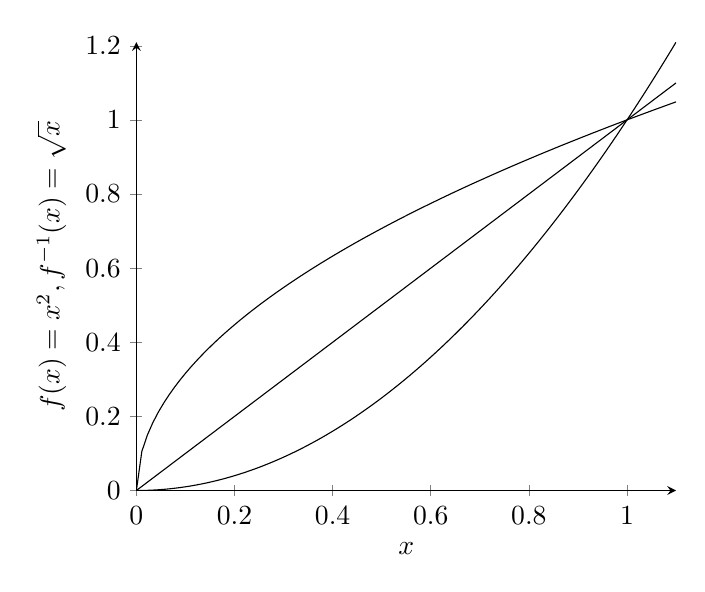
\begin{tikzpicture}
     \begin{axis}[axis lines = left, xlabel = $x$, ylabel = {$f(x)=x^2, f^{-1}(x)=\sqrt{x}$}]
%Below the red parabola is defined
     \addplot [domain=0:1.1, samples=100]{x^2};
     \addplot [domain=0:1.1, samples=100]{x^0.5};
     \addplot [domain=0:1.1, samples=100]{x};
     %\addlegendentry{$f(x)=\exp(x)$}
     \end{axis}
  \end{tikzpicture}
  \caption{$f(x)$ and $f^{-1}(x)$ are symmetric about $y=x$}
  \setfloatalignment{b}
\end{marginfigure}
A specific example is the function $f(x)=x^2$ and it can be easily seen that $\sqrt{x}$ \textit{reverses} $x^2 ~\forall~x~\in~[0,\infty] $ and therefore, $f^{-1}(x)=\sqrt{x}$. Geometrically, this can be seen as $f(x)$ and $f^{-1}(x)$ are symmetric about the diagonal $y=x$ since the input and output reverses their role. We can also prove it from the definition of what the \textit{inverse} has to satisfy, that is, $\sqrt{x^2}=x$ or, $(\sqrt{x})^2=x$ $\forall~x~\in~[0,\infty]$.

\newthought{Polynomials} are a very important class of functions in calculus generally expressed as $P(x) = C_0 + C_1x + \cdots + C_nx^n$. The largest power of $x$ is called the \textit{degree} of the polynomial. The summation notation of polynomials as $\sum_{k=0}^n C_kx^k$ makes it a very simple way of writing it out. The $C_k$ are constants known as the \textit{coefficients} of the polynomials.